\subsection{Interference scenario}
\label{interference}
\subsubsection{Can subdermal GPS microchips enable human tracking?}
The feasibility of receiving GNSS signals through human skin is severely limited due to the signal's extremely weak power and the radio-frequency (RF) attenuation properties, especially in the L-band, of biological tissue. 

GNSS signals are very weak and require a line-of-sight to satellites. Human tissue, with its high water and organic content, strongly attenuates these signals such that subdermal reception is extremely unlikely without an external antenna.

\subsubsection{Using minced pork to simulate human tissues for GNSS signal attenuation}
We employed minced pork as a biological analog to human tissues to investigate the attenuation of GNSS signals in subdermal environments. Porcine meat is widely recognized in biomedical research as a suitable surrogate for human tissues due to its comparable physiological and dielectric characteristics \cite{ranamukhaarachchi2016micromechanical}. In addition, it offers a homogeneous medium that facilitates consistent and reproducible measurements. However, while it simplifies experimental conditions, this model lacks the stratified structure of natural skin, which may influence the attenuation characteristics compared to intact tissues.
% By utilizing minced pork, we aim to establish a baseline understanding of how biological tissues can affect the reception of GNSS signals by subdermally implanted devices. This approach allows for controlled experimentation while acknowledging the limitations inherent in the model.

\subsubsection{Scenario analysis}
For this experiment, we replicated the same conditions previously described in \ref{sec:opensky}, maintaining a continuous clock signal without discontinuities. The measurements were repeated the following day at the same time (20:16:32 UTC+2), this time surrounding the device \cite{samsungs23ultra} with a 2.5 cm thick layer of minced pork to simulate subdermal tissue.

To evaluate the effect of biological interference on GNSS signal quality, we compared the Horizontal Dilution of Precision (HDOP) and the number of tracked satellites across two scenarios. In the interference scenario (\ref{fig:carne_hdop}), HDOP values fluctuate noticeably, ranging approximately from 0.9 to 1.4, and the number of SATs varies frequently between 6 and 9. These fluctuations indicate unstable satellite geometry and occasional signal degradation, likely due to the RF attenuation properties of the biological tissue. The increased HDOP and reduced satellite availability correlate with potential deterioration in positional accuracy, consistent with expected GNSS performance under obstructed conditions.
In contrast, in open-sky conditions, the GNSS receiver can maintain high positioning accuracy with minimal dilution effects, as already discussed in (\ref{sec:opensky}).


\begin{figure}[H]
    \centering
    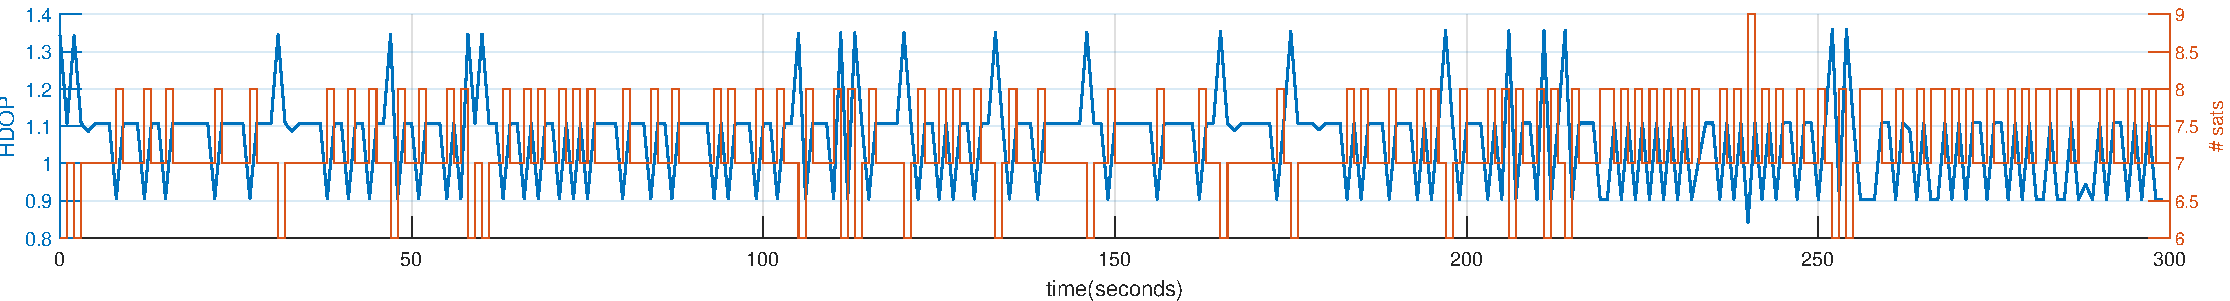
\includegraphics[width=1.00
    \linewidth]{images/carne_hdop_carne.pdf}
    \caption{HDOP and SATs number in the interference scenario}
    \label{fig:carne_hdop}
\end{figure}

\begin{figure}[H]
    \centering
    \begin{minipage}[b]{0.48\linewidth}
        \centering
        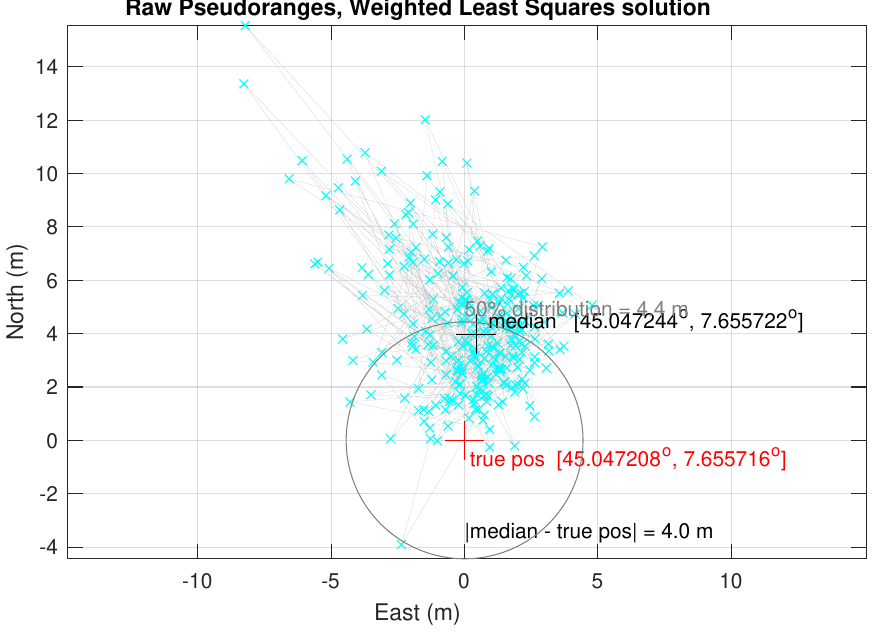
\includegraphics[width=\linewidth]{images/carne_pos.png}
        
        \caption{Positioning in the interference scenario}
        \label{fig:carne_pos}
    \end{minipage}
    \hfill
    \begin{minipage}[b]{0.48\linewidth}
        \centering
        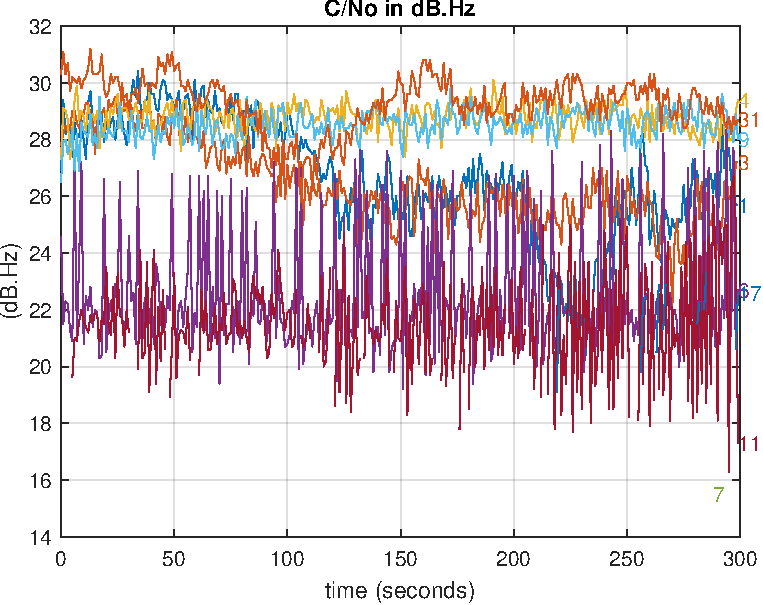
\includegraphics[width=\linewidth]{images/carne_CN0_carne.pdf}
        \caption{C/N0, dB-Hz in the interference scenario}
        \label{fig:CN0_carne}
    \end{minipage}
\end{figure}

Figures \ref{fig:CN0_punto_3} and \ref{fig:CN0_carne} show the Carrier-to-Noise Density Ratio (\(C/N_0\)) measurements under the two conditions, a key indicator of GNSS signal strength and quality, with higher values correlating to better measurement reliability and accuracy. In the interference scenario, most satellite signals exhibit significant attenuation, with \(C/N_0\) values ranging predominantly between 20–30 dB-Hz. The lower and more fluctuating values suggest substantial signal degradation caused by the dielectric absorption and scattering effects of biological tissue. In contrast, in the non-interference scenario, \(C/N_0\) values are consistently higher and less variable, mostly within the 35–50 dB-Hz range, indicating robust and stable signal reception. 

The observed differences between the two conditions provide clear experimental evidence that biological tissue attenuates GNSS signals, reducing the number and the geometry of usable satellites and potentially compromising positioning accuracy. 
% These findings underscore the practical limitations of subdermal GNSS implantation without an external antenna or signal relay mechanism.

In Figure \ref{fig:carne_pos}, we observe an interesting outcome: although measurements are generally more precise in the open-sky scenario (fig. \ref{fig:pos_punto_3_precision}), the results in the interference setting show a median only 4 m away from the real position. This may be due to a sort of filtering effect of the biological material, which limits the number of usable satellites to the ones that had a stronger and more stable signal.

However, this apparent gain in accuracy does not correlate to a better precision (fig. \ref{fig:accPos}), as the various position states appear more scattered (see also fig. \ref{fig:carne_pos_precision}), suggesting that biological tissue introduced biases due to signal weakening and poor satellite geometry (HDOP). Therefore, in applications requiring both high accuracy and reliability, biological interference must be considered a non-negligible source of error, reinforcing the impracticality of using unassisted subdermal GNSS devices for precise human tracking.